% it/figures/literature/cleveland_hierarchy.tex — versione italiana
\begin{figure}[!ht]
    \centering
    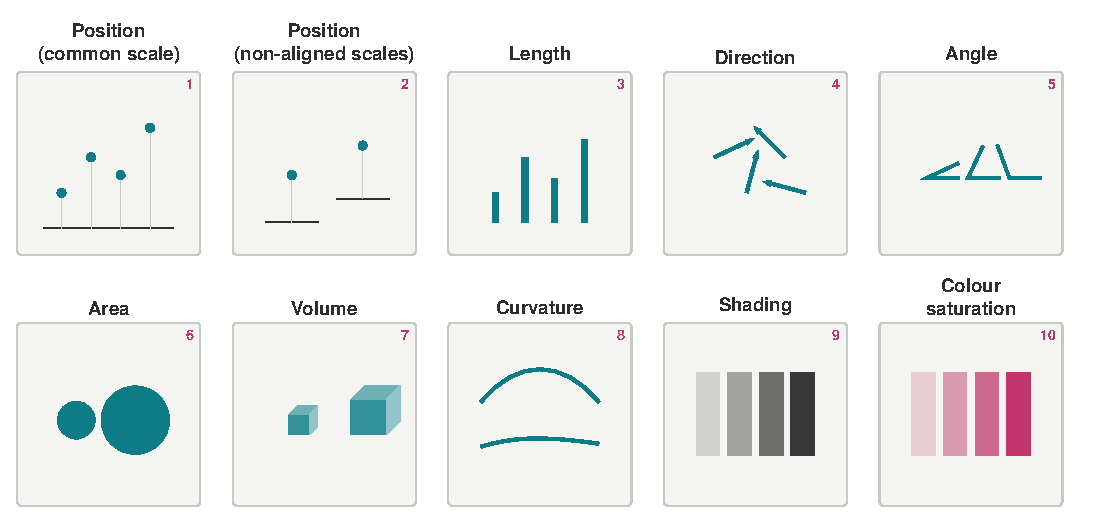
\includegraphics[width=\textwidth]{figures/literature/cleveland_preview.pdf}
    \caption[La gerarchia dei compiti percettivi di Cleveland \& McGill.]{\textbf{La
    gerarchia dei compiti percettivi elementari, secondo \citet{clevelandmcgill1984}.}
    Le codifiche sono ordinate per accuratezza di decodifica, dalla più accurata (1,
    posizione su una scala comune) alla meno accurata (10, saturazione del colore).
    L'ordinamento è empirico, non estetico: riflette quanto accuratamente le persone
    estraggono un valore quantitativo da ciascun canale visivo. Sta alla base del
    principio~P0 della grammatica di design (Tabella~\ref{tab:design-grammar}) ---
    assegnare la variabile più importante al canale decodificato più accuratamente ---
    e del principio~P1, che colloca la magnitudine continua sulla posizione spaziale.}
    \label{fig:perceptual-hierarchy}
\end{figure}
